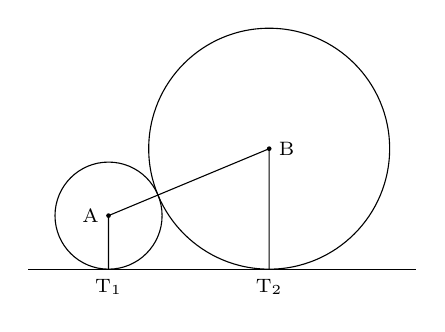
\begin{tikzpicture}[scale=0.17]
\coordinate (A) at (0,4); \coordinate (B) at (12,9);
\draw (A) circle (4); \draw (B) circle (9); \draw (-6,0)--(23,0);
\draw (A)--(B) (A)--(0,0) (B)--(12,0);
\fill (A) circle (5pt) (B) circle (5pt);
\node[left] at (A){\scriptsize A}; \node[right] at (B){\scriptsize B};
\node[below] at (0,0){\scriptsize $\mathrm T_1$}; \node[below] at (12,0){\scriptsize $\mathrm T_2$};
\end{tikzpicture}